\documentclass[10pt,twocolumn,letterpaper]{article}

\usepackage{cvpr}
\usepackage{times}
\usepackage{epsfig}
\usepackage{graphicx}
\usepackage{amsmath}
\usepackage{amssymb}
\usepackage{array}
\usepackage{xfrac}
\usepackage{amssymb}
%\usepackage{todonotes}
\usepackage{centernot}
\usepackage{textcomp}
\usepackage{blindtext}
\usepackage{centernot}
\usepackage{wasysym}
\usepackage{siunitx}
\usepackage[letterpaper]{geometry}
\usepackage{color}
%\usepackage[table]{xcolor}
\usepackage{amsfonts}
\usepackage{mathtools}
\usepackage{multirow}
\usepackage[small,it]{caption}
%\usepackage{titling}
%\usepackage{filecontents}
%\usepackage{titlesec}
\usepackage[section]{placeins}
%\usepackage[hidelinks]{hyperref}
%\usepackage{fancyhdr}
\usepackage{cancel}
%\usepackage{abstract}
\usepackage{minted}
\usepackage{widetext}
\usepackage[utf8]{inputenc}

\sisetup{output-exponent-marker=\textsc{e}}

\DeclareMathOperator*{\argmax}{arg\,max}
\DeclareMathOperator*{\argmin}{arg\,min}

\newcommand{\squishlist}{
 \begin{list}{$\bullet$}
  { \setlength{\itemsep}{0pt}
     \setlength{\parsep}{3pt}
     \setlength{\topsep}{3pt}
     \setlength{\partopsep}{0pt}
     \setlength{\leftmargin}{1.5em}
     \setlength{\labelwidth}{1em}
     \setlength{\labelsep}{0.5em} } }


\newcommand{\squishlisttwo}{
 \begin{list}{$\bullet$}
  { \setlength{\itemsep}{0pt}
    \setlength{\parsep}{0pt}
    \setlength{\topsep}{0pt}
    \setlength{\partopsep}{0pt}
    \setlength{\leftmargin}{2em}
    \setlength{\labelwidth}{1.5em}
    \setlength{\labelsep}{0.5em} } }

\newcommand{\squishend}{
  \end{list}  }
\footskip = 50pt
\setlength{\skip\footins}{10pt}

\newcommand*{\vertbar}{\rule[-1ex]{0.5pt}{3.0ex}}
\newcommand*{\horzbar}{\rule[.5ex]{2.5ex}{0.5pt}}

% Include other packages here, before hyperref.

% If you comment hyperref and then uncomment it, you should delete
% egpaper.aux before re-running latex.  (Or just hit 'q' on the first latex
% run, let it finish, and you should be clear).
\usepackage[breaklinks=true,bookmarks=false]{hyperref}

\cvprfinalcopy % *** Uncomment this line for the final submission

\def\cvprPaperID{****} % *** Enter the CVPR Paper ID here
\def\httilde{\mbox{\tt\raisebox{-.5ex}{\symbol{126}}}}

% Pages are numbered in submission mode, and unnumbered in camera-ready
%\ifcvprfinal\pagestyle{empty}\fi
\setcounter{page}{1}
\begin{document}

%%%%%%%%% TITLE
\title{Evaluation of segmentation methods based on the BSDS500 benchmark}

\author{Edgar A. Margffoy-Tuay\\
Universidad de los Andes\\
201412566\\
{\tt\small ea.margffoy10@uniandes.edu.co}
% For a paper whose authors are all at the same institution,
% omit the following lines up until the closing ``}''.
% Additional authors and addresses can be added with ``\and'',
% just like the second author.
% To save space, use either the email address or home page, not both
%\and
%Second Author\\
%Institution2\\
%First line of institution2 address\\
%{\tt\small secondauthor@i2.org}
}

\maketitle
%\thispagestyle{empty}

%%%%%%%%% ABSTRACT
\begin{abstract}
To evaluate a set of algorithms designed to solve a specific problem of interest, it is essential to define a common ground of evaluation, such as defining a dataset proposed to evaluate the problem, this database shall contain a set of inputs, labels and a evaluation methodology that allows different teams to compare their solutions to the problem to other proposals. In the present document, we pretend to introduce the Berkeley Segmentation Dataset and Benchmarks (BSDS500) as a framework to evaluate the performance of different segmentation algorithms, and more specifically, we compare the performance of different unsupervised segmentation algorithms, like k-means, watershed and UCM, by comparing their results on the Precision-Recall curve defined on BSDS500.
\end{abstract}

%Segmentation represents one of the core Computer Vision tasks in scientfic and academic research since the 1970s, this problem is defined as the grouping of pixels on a image according to several semantic categories of interest. Until recently, this problem was approached by using pixel-level mathematical formulations based on classical image processing and DSP, without any association with other Computer Vision problems nor any AI-related task, such as NLP. However, after the rise of

%%%%%%%%% BODY TEXT
\section{Introduction}
%\subsection*{Context}
Before the introduction of normalized benchmarks to evaluate the performance of different algorithms proposed to solve an specific task, each research team chose a set of predefined catalog images, on which, the proposed method results were evaluated and presented, this evaluation pipeline represented a challenge when different segmentation algorithms were to be compared and tested against, which prompted an uneven challenge between the different teams. To account for this difficulties, it was essential to define a benchmark that provides a set of uniform and public images with their respective labels and annotations, along with the dataset, an evaluation methodology must be provided, this framework allows to compare and classify different algorithms on a common ground. 
\\
\\
On image segmentation context, the preferred benchmark was proposed by the Computer Vision Group at UC Berkeley, their database (BSDS500) \cite{amfm_pami2011}, consisted of 500 images (Photographs), which were labeled by different humans. All the segmentations defined on the database have different boundary and region precision, \textit{i.e.,} There are more or less defined regions per mask annotation. This allows to evaluate the segmentation using the Precision-Recall curve and the $F_1$ score statistic, which in turn can be compared with the Human score evaluated over the image segmentation task.

\section{Materials and Methods}

%\begin{figure*}[t]
%	\centering
%	%	\begin{center}
%	%\fbox{\rule{0pt}{2in} \rule{0.9\linewidth}{0pt}}
%	\epsfig{file=./Assets/Model_red.pdf,width=0.8\linewidth,clip=}
%	%\includegraphics[width=0.8\linewidth]{egfigure.eps}
%	%	\end{center}
%	\caption{Visual description of the planned baseline to approach the image segmentation recovery problem given a video input. Images taken by the author}
%	\label{Fig:F1}
%	%\label{fig:long}
%	%\label{fig:onecol}
%\end{figure*}

On the present document, a comparison of different unsupervised segmentation methods is proposed, based on  the BSDS500 benchmark evaluation pipeline, the methods to be compared against correspond to k-means and Ultrametric Contour Maps, each model parameters are setup based on the results obtained after the heuristic evaluation done over a subset of 20 images of the dataset, the evaluation score was different from the evaluation methodology proposed by the UC Berkeley team (Precision/Recall) and was based on contour comparison of the results against the ground truth contour masks. Now the results are evaluated over all the test set of BSDS500 dataset, using the fast morphological benchmark, which compares the boundary reconstruction of each image by using the segmentation morphological reconstruction of the ground truth boundary masks. To represent the input images, each input vector was represented as a coordinate on Lab space, with spatial information. The initial parameters were evaluated over the validation and training sets of the database, the chosen number of segmentation regions correspond to 5, 10, 20, 50 and 100, mapping to 5 points on the AP curve respectively. With respect to the watershed    
\\
\\
The implementation of the watershed procedure is based on the OpenCV\footnote{\url{http://opencv.org}} Python bindings, with the regional minima extraction routines adapted from the Gala library\footnote{\url{https://github.com/janelia-flyem/gala}}, the clustering methods are based on the Sckit-learn\footnote{\url{http://scikit-learn.org/stable/}} implementations. Also, the centroid and means initialization for K-Means was based on the KMC$^{2}$\footnote{\url{https://github.com/obachem/kmc2}} algorithm \cite{Bachem:2016:AKS:3016100.3016103}, all the routines were implemented on Cython, to improve execution times and the efficiency of the evaluation procedure.



\subsection*{About the models}

\subsubsection*{Watershed Transform}
The watershed transform is based on the concept of watershed lines, these lines correspond to the local basin in which all drops of water are gathered when they fall down from a peak. In this context, the peaks of the images correspond to contours, and the space between borders may correspond to a river basin, the idea of the algorithm is to flood the image from the river basins (Regional minima), up to the peaks, at the end of the procedure, only the peaks remain, which implies that a boundary segmentation of the image is achieved. However, due to the existance of multiple regional minima on the gradient, this method is prone to produce an oversegmentation of the image, to overcome this limitation, it is possible to define a set of precomputed markers and impose them over the image, by executing this procedure, the flooding is not done over the set of markers, reducing the oversegmentation on the image. Due to the inexistance of precomputed markers over each image, the markers are selected as the regional minima of height $h$ (h-minima), the value of $h$ is increased, starting on 0, until the total number of regions is equal to $K$.

\subsubsection*{K-Means}
In the present experiment, K-Means was employed to segment an image by conforming clusters from pixel information, the clusters means were calculated by using the $\ell_2$ distance metric (Euclidean), which gives rise to spherical and convex color clusters, which can be spatially sparse or localized, depending on the inclusion of spatial information. To segment an input image, for each color triplet, the label of the closest mean is assigned, finally, the segmented image is reshaped into the image original dimensions.
 

\subsubsection*{Ultrametric Contour Maps}
The Ultrametric Contour Maps is a hierarchical segmentation representation based on the Ultrametric Distance, it groups a set of different segmentations, based on the region contours and a similarity function between adjacent regions. This similarity distance must comply with the ultrametric inequality, for instance, a distance between points on Lab$^{*}$ space can be define as a mesure of disimilarity of regions on the hierarchy, this definition allows to refine the contour detection and segmentation of an image. Also, UCM compiles all the segmentation trees on a single contour image, which can be thresholded to extract each of the individual segmentation levels present on the ultrametric dendrogram.

\section{Results}
Before the evaluation of all segmentation methods, it was expected that UCM outperforms the performance of both k-means and watersheds, due to the expressivity implied by using a segmentation hierarchy family instead of a single segmentation, this approach guarantees that more information is captured on a single image, compared to the clustering based approaches, such as K-Means or morphological methods like watersheds, that do not take in account more relations among pixels and regions and are very limited. Among the strengths of UCM we can found, it is that the ultrametric distance between regions impose more restrictions and conditions that the regions must comply in order to be merged, those restrictions expressed in terms of color, border and distance affinity can be regularized and controlled via hyperparameters, which can fine-tune the results of the method.
\\
\\
On the other hand, the hyperparameters defined on the clustering methods, \textit{i.e.,} $K$, just only define the number of segmentation regions to be found, however, this parameter does not define or expresses how these regions should be found. This limitation accounts to the fact that unsupervised segmentation methods, such as k-means are based on the fact that grouping should be defined and built upon a distance that relates the elements on the image space, nevertheless, there does not exists a deterministic schema to define the representation of each point and the distance definition between each point on that space. In conclusion, is not possible to regularize nor guide the segmentation process if those methods are to be used.
\\
\\
As it can be seen on Figures~\ref{Fig:F1} and \ref{Fig:F2}, the overall PR\footnote{In the present benchmark, it is desired that the $F_1$ score approximates or overshoots the human performance (0.79) and approximate to the value 1, on which all instances are segmented correctly (Precision) and no correct segmentation is missed (Recall)} curve comparison between the previously defined methods allows to draw the same conclusion as the exposed previously, in this case, the UCM performance is far from better than the results obtained after evaluating the PR scores for k-means, as it can be inferred of the benchmark evaluation statistics (Table~\ref{Tab:T1}), by which, the k-means $F_1$ score (0.54) is approximately lesser on 20\% than the score obtained after evaluating UCM (0.73). This implies that UCM outeperforms k-means, due to the expressive and rich hierarchical representation, which adapt to the different segmenation levels and thresholds and segmentation families according tho the ultrametric distance and the dissimilarity measure between regions, which increases both Precision and Recalled, compared to K-means, which present an avaerage Recal but a low precision, which means that none of the segmentation boundaries are lost, but the segmentation proposed does not right. It is worth to notice that evaluating Watershed performance was difficult due to the uniform evaluation of the number of regions chosen on each image, \textit{i.e.,} Some images could present 1000 regions, but others only 999 regions, effect that renders the comparison useless and biased against a subset of the values subject to evaluation, and therefore, the results were not subject to comparison.

\begin{table}[H]
	\centering
	\begin{tabular}{|c|c|c|c|}
		\hline
		Method & ODS & OIS & AP \\ \hline
		\textbf{UCM} & 0.73 & 0.76 & 0.72 \\ \hline
		K-Means & 0.54 & 0.57 & 0.3 \\ \hline
	\end{tabular}
\caption{Precision - Recall evaluation results on BSDS500 of UCM and K-means over the test set}
\label{Tab:T1}
\end{table}

\begin{figure}[H]
	\centering
	%	\begin{center}
%	%\fbox{\rule{0pt}{2in} \rule{0.9\linewidth}{0pt}}
	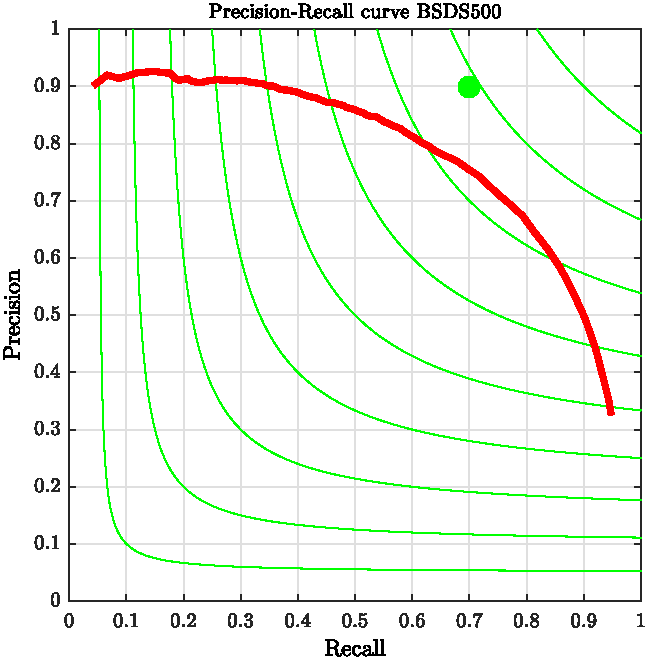
\epsfig{file=./Assets/ucm2.pdf,width=1.0\linewidth,clip=}
%	%\includegraphics[width=0.8\linewidth]{egfigure.eps}
%	%	\end{center}
	\caption{Precision-Recall curve results associated to UCM evaluation over BSDS500 test set}
	\label{Fig:F1}
\end{figure}

\begin{figure}[H]
	\centering
	%	\begin{center}
	%	%\fbox{\rule{0pt}{2in} \rule{0.9\linewidth}{0pt}}
	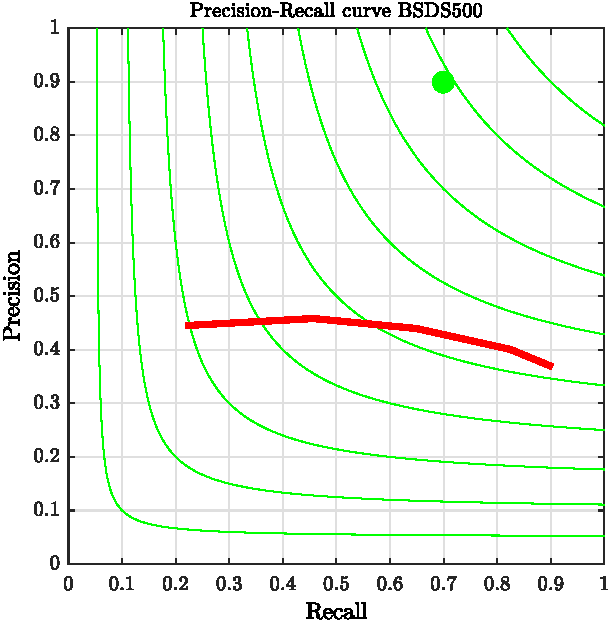
\epsfig{file=./Assets/k-means.pdf,width=1.0\linewidth,clip=}
	%	%\includegraphics[width=0.8\linewidth]{egfigure.eps}
	%	%	\end{center}
	\caption{Precision-Recall curve results associated to K-means (Lab+xy) evaluation over BSDS500 test set}
	\label{Fig:F2}
\end{figure}


\section{Conclusions}
After evaluating different unsupervised segmentation methods, it is possible to appreciate that those that have more regularization parameters, present more refined segmentation regions and boundary contours, due to the definition of higher-level distance metrics and similarity measures between groups of pixels, increasing the number of parameters and affinities allows us to improve the overall result when a method is evaluating on a common ground benchmark like BSDS500. The methods based only on clustering are limited in terms of regularization and control of the segmentation regions to define, \textit{i.e.,} It is no possible to guide the segmentation regions that shall result after applying one of those methods, also, the computational time complexity increases if the number of desired regions increases, which only decreases the overall accuracy score on the PR curve. Finally, the models that exploit the expressiveness of a hierarchical segmentation approach can capture more information, and therefore present a better performance when subject to evaluation on different benchmarks, like BSDS500. To improve the accuracy of some of the clustering methods, it should be possible to enrich and extend the representation space of each pixel on the image and the distance definition between groups as well, however this shall increase the time complexity and may not approximate to better and expressive models, such as UCM. 


{\small
\bibliographystyle{ieee}
\bibliography{egbib}
}


\newpage
%\section{Some Results}
%\begin{figure}[H]
%	\centering
%	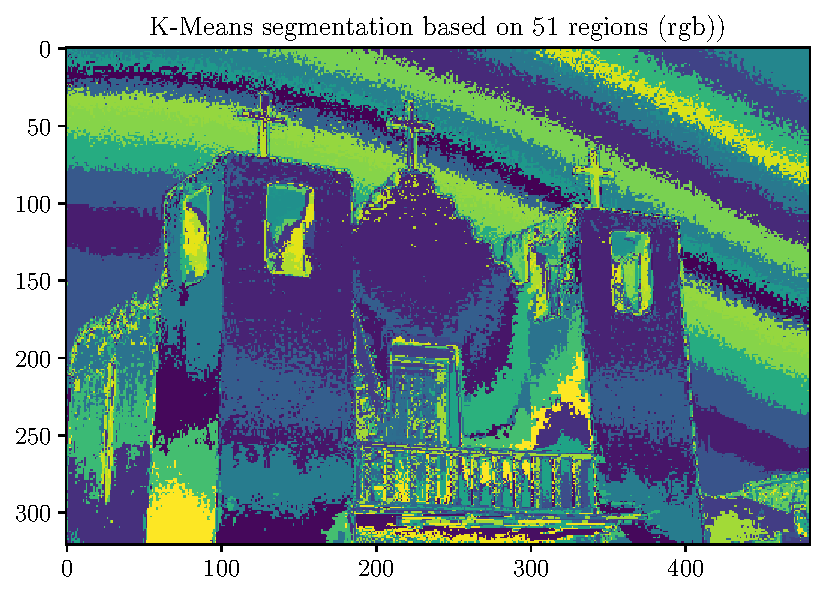
\epsfig{file=./Assets/24063_k-means_rgb_51.pdf,width=1.0\linewidth,clip=}
%	\caption{Example of K-Means segmentation result subject to 51 regions (No spatial)}
%	\label{Fig:kmeans1}
%\end{figure}
%
%
%\begin{figure}[H]
%	\centering
%	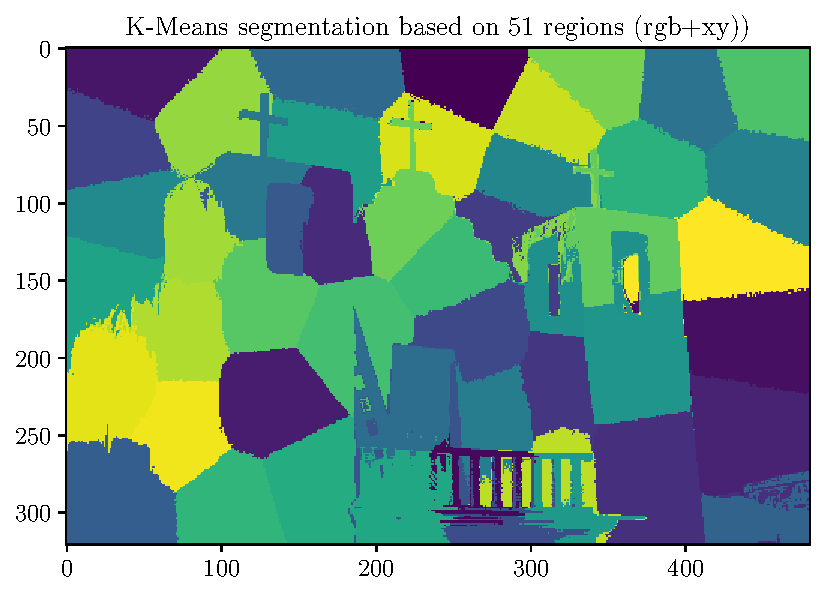
\epsfig{file=./Assets/24063_k-means_rgb+xy_51.pdf,width=1.0\linewidth,clip=}
%	\caption{Example of K-Means segmentation result subject to 51 regions (Spatial), this figure presents a large number of convex and spherical regions}
%	\label{Fig:kmeans2}
%\end{figure}
%
%\begin{figure}[H]
%	\centering
%	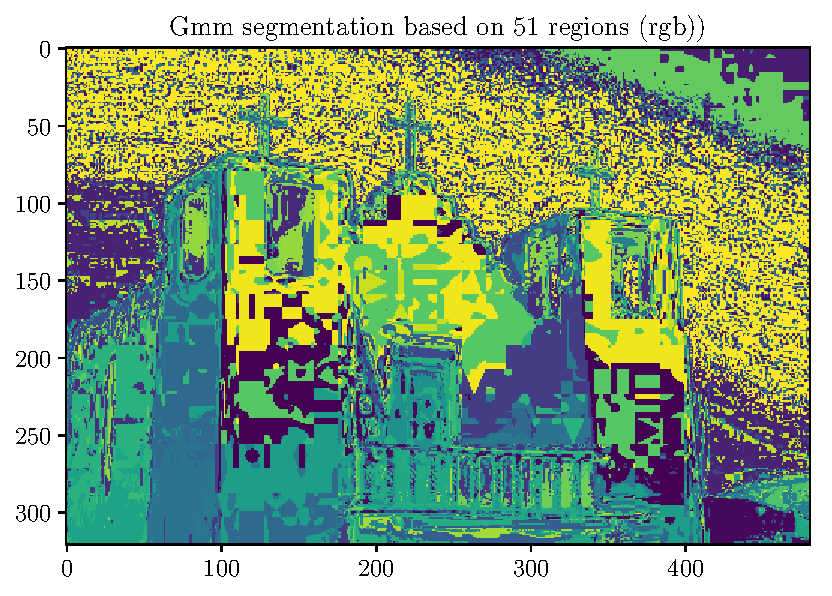
\epsfig{file=./Assets/24063_gmm_rgb_51.pdf,width=1.0\linewidth,clip=}
%	\caption{Example of GMM segmentation result subject to 51 regions (No spatial)}
%	\label{Fig:gmm1}
%\end{figure}
%
%\begin{figure}[H]
%	\centering
%	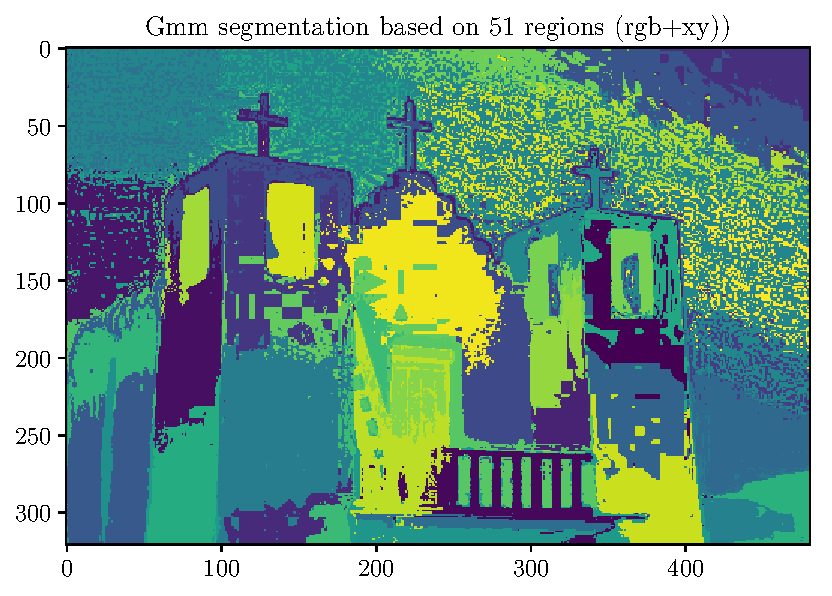
\epsfig{file=./Assets/24063_gmm_rgb+xy_51.pdf,width=1.0\linewidth,clip=}
%	\caption{Example of GMM segmentation result subject to 51 regions (Spatial information added), the noise was reduced}
%	\label{Fig:gmm2}
%\end{figure}
%
%\begin{figure}[H]
%	\centering
%	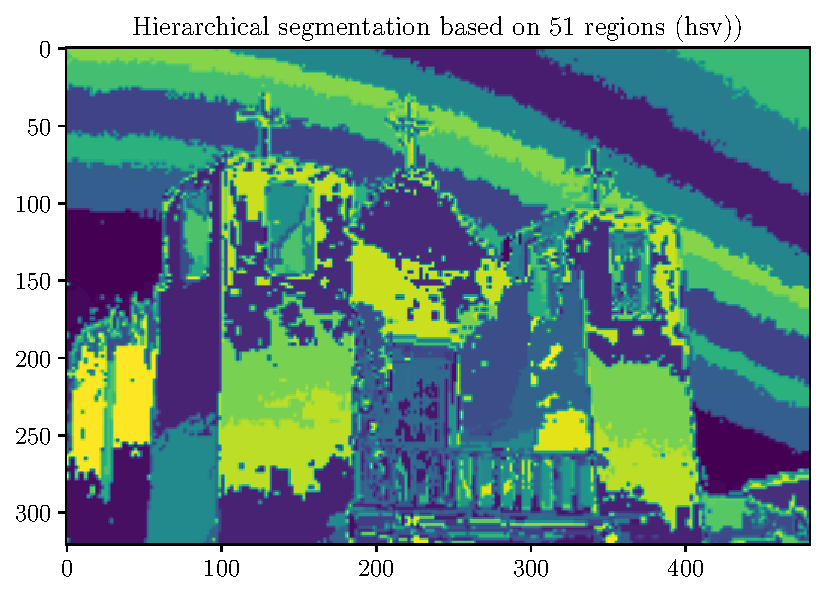
\epsfig{file=./Assets/24063_hierarchical_hsv_51.pdf,width=1.0\linewidth,clip=}
%	\caption{Example of Hierarchic segmentation result subject to 51 regions (No spatial information added), notice the smooth noise throughout all the regions by interpolation effects}
%	\label{Fig:hier1}
%\end{figure}
%
%\begin{figure}[H]
%	\centering
%	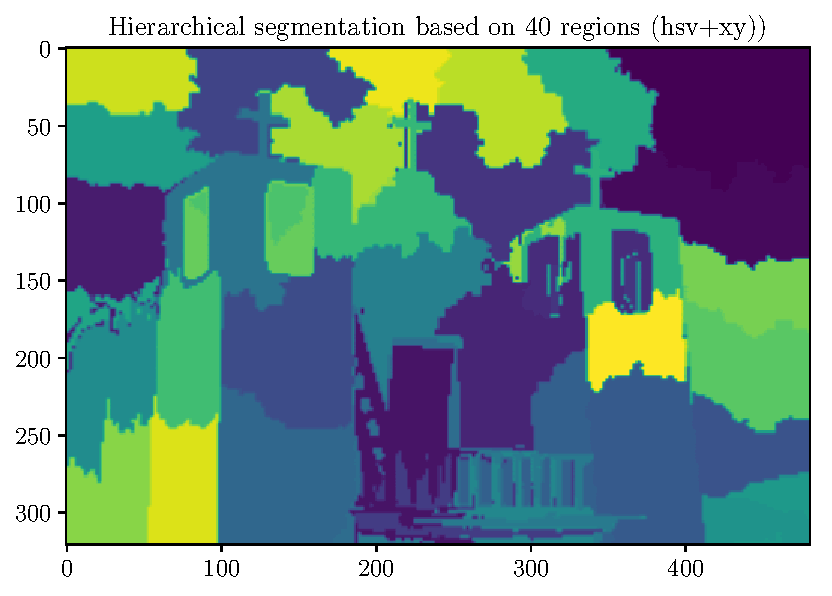
\epsfig{file=./Assets/24063_hierarchical_hsv+xy_40.pdf,width=1.0\linewidth,clip=}
%	\caption{Example of Hierarchic segmentation result subject to 40 regions (Spatial information added), notice the smooth noise throughout all the regions by interpolation effects}
%	\label{Fig:hier2}
%\end{figure}
%
%\begin{figure}[H]
%	\centering
%	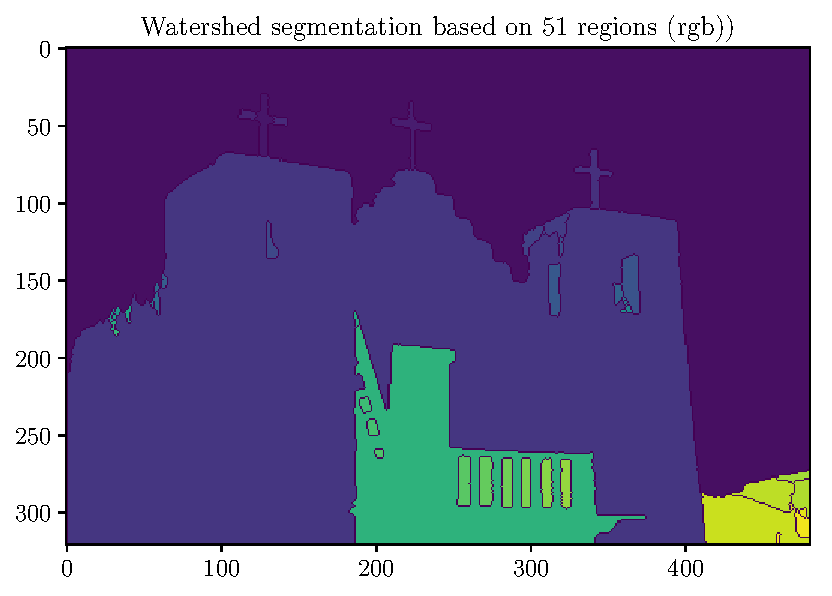
\epsfig{file=./Assets/24063_watershed_rgb_51.pdf,width=1.0\linewidth,clip=}
%	\caption{Example of H-Minima Watershed segmentation result subject to 51 regions, notice the well defined contours and regions}
%	\label{Fig:water1}
%\end{figure}
%
%\begin{figure}[H]
%	\centering
%	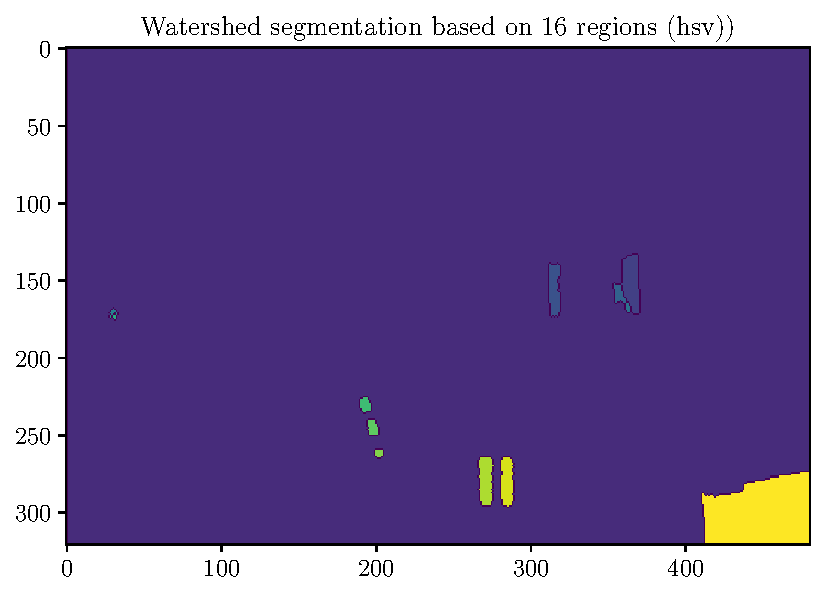
\epsfig{file=./Assets/24063_watershed_hsv_16.pdf,width=1.0\linewidth,clip=}
%	\caption{Example of H-Minima Watershed segmentation result subject to 16 regions, notice the disappearance of the main ROI}
%	\label{Fig:water2}
%\end{figure}



\end{document}
